\subsection{Ключевые эксперименты}

\subsubsection{Опыт Резерфорда по рассеянию $\alpha$-частиц}
%ref: ципенюк, 96
{\footnotesize
  \textsc{Справка.} \emph{Дифференциальным сечением рассеяния} называется
  отношение числа частиц, рассеянных за единицу времени в элемент телесного угла
  $ d\Omega = \sin\theta\,d\varphi d\theta $, к плотности потока падающих частиц
  $ nv $, где $ n $ есть плотность частиц, а $ v $ --- их скорость. 

  \emph{Классическая модель Томпсона}. Требовалось объяснить нейтральность атома,
  несмотря на присутствие электронов. В этой модели электроны свободно плавают в некотором
  равномерно положительно заряженном облаке. Они не могут вылететь наружу, поскольку
  снаружи меньше положительного заряда, чем внутри.

  При распаде некоторых радиоактивных веществ испускаются \emph{$ \alpha
  $-частицы} --- положительно заряженные частицы, образованные двумя протонами и
  двумя нейтронами; ядро атома гелия.
}



Размышления основаны на классической физике. От радиоактивного источника $ \alpha $-частицы пропускались через узкое
отверстие, после чего пучок попадал на фотопластинку и давал на ней чёткое
изображение щели. Было замечено, что происходит \emph{рассеивание\footnote{То
  есть отдельные $ \alpha $-частицы отклоняются в движении.} $ \alpha
$-частиц}, то есть размытие полученного изображения, если заполнить место
проведения опыта --- вакуумную стеклянную полость --- газом. 

Даже для небольшого отклонения $ \alpha $-частицы потребовалась бы большая сила,
которой было неоткуда взяться в электрически нейтральной в среднем модели
Томпсона. 

Ученики Резерфорда поставили на пути пучка тонкую фольгу. Ими было обнаружено,
что угол отклонения $ \alpha $-частицы может (в одном случае из 8000 для
платиновой фольги) достигать величины,
близкой к $ 180^\circ $. Такое отклонение имеет вероятность
порядка $ 10^{-3500} $, если предположить многократное рассеивание в модели
Томпсона. Поскольку сильный эффект наблюдался редко, было предположено, что основную часть атома занимает пустота, а в
малом объёме находится массивное \emph{ядро атома}, а частица отклоняется
вследствие одного взаимодействия с этим ядром, чья масса много больше массы
$ \alpha $-частицы.

Будем рассматривать движение частицы относительно неподвижного массивного
центра. Её траекторией тогда будет гипербола (сочтём этот факт известным) с фокусом $ M $ (см. рисунок
\ref{fig:reser1}).
\begin{wrapfigure}{l}{0.4\textwidth}
	\centering
	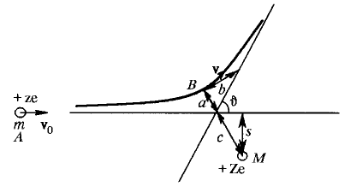
\includegraphics[width=0.4\textwidth]{img/oral-05/reser1.png}
  \caption{}
  \label{fig:reser1}
\end{wrapfigure}
Законы сохранения энергии и момента количества движения, если частица $ m $
последовательно находится в положениях $ A $ и $ B $, и закон Кулона непосредственно дают 
\begin{align*}
  \frac{1}{2} mv_0^2 &= \frac{1}{2}mv^2 + \frac{zZe^2}{a+c},\\
    mv_0s&=mv(a+c).
\end{align*}
На основании свойств гиперболы имеем\footnote{Из свойства гиперболы $ c^2 = a^2
  + b^2$, что влечёт равенство соответствующих треугольников и остальные два
соотношения.}
\begin{gather*}
    s = b, \quad c^2=a^2+b^2, \quad \tg \frac{\vartheta}{2} = \frac{a}{b},\\
    \tg \frac{\vartheta}{2} = \frac{zZe^2}{smv_0^2}.
\end{gather*}
\begin{wrapfigure}{r}{0.4\textwidth}
	\centering
	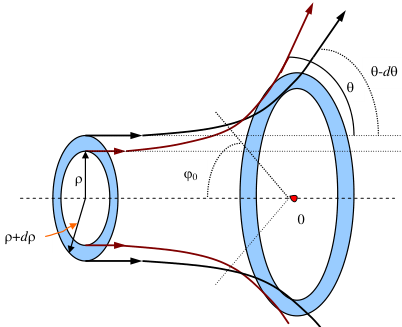
\includegraphics[width=0.4\textwidth]{img/oral-05/reser2.png}
  \caption{Рассеяние частиц с прицельным расстоянием $ \rho $.}
  \label{fig:reser2}
\end{wrapfigure}
Отсюда видно, что все частицы, попадающие в круговой слой $s $ и
$s + ds$, будут рассеиваться в угловом интервале $ \vartheta, \vartheta+d\vartheta $. Это
означает, что выделенная у ядра-мишени поверхность $ 2\pi s\,ds $ является
\emph{дифференциально эффективным сечением $ d\sigma $}. Поэтому с учётом  
\[
    |ds| = \frac{zZe^2}{mv_0^2}
    \frac{1}{\sin^2(\vartheta/2)}\frac{1}{2}\,d\vartheta
\]
мы получаем 
\[
    d\sigma = 2\pi \left( \frac{zZe^2}{mv_0^2} \right)^2
    \frac{1}{2}\frac{d\vartheta}{\tg(\vartheta/2) \sin^2 (\vartheta/2)}.
\]
Учитывая, что $ d\Omega = 2\pi\sin\vartheta\,d\vartheta $, мы окончательно
получаем 
\[
    d\sigma = \left( \frac{zZe^2}{2mv_0^2} \right)^2
    \frac{d\Omega}{\sin^4(\vartheta/2)}.
\]
Это и есть \emph{формула Резерфорда}. Отклонения от неё наблюдаются только для
очень малых углов рассеяния и для углов, близких к $ \pi $. Вскоре было
установлено, что электрический заряд центрального ядра в точности равен
номеру данного элемента в периодической таблице Менделеева.
Размер ядра $ \approx 10^{-12} $\,см, а размер орбиты\footnote{Позже выяснилось,
что никаких орбит не существует.} электронов $ \approx 10^{-8} $\,см.

\textsc{Несоответствие классической модели.} Летая по орбите, электрон имеет
ускорение. Значит, он должен выпускать световые волны и терять свою энергию. В
конце концов он должен был бы упать на ядро атома.






\subsubsection{Измерение спектра излучения АЧТ}
Будем исходить из формулы \eqref{eq:mods}. Спектральная плотность равна
\[
  u_{\omega, T}\,d\omega = \frac{dN\cdot\langle \varepsilon \rangle}{V} =
  \frac{\omega^2}{\pi^2 c^3}\langle \varepsilon \rangle,
\]
где $ \langle \varepsilon \rangle $ --- средняя энергия волны частоты $ \omega
$. Согласно классической теореме о равномерном распределении энергии по степеням
свободы, в состоянии термодинамического равновесия на каждую степень свободы
системы\footnote{Их в данном случае две: магнитная и электрическая.} приходится
в среднем энергия $ kT/2 $, где $ k $ --- постоянная Планка. Выше была получена
формула, позволяющая найти испускательную способность АЧТ в виде 
\[
  r^\ast_{\omega, T} = \frac{\omega^2}{4\pi^2 c^2}kT.
\]
Эта формула носит имя \emph{формулы Рэлея -- Джинса}. Опыты резко расходятся с ней
при больших длинах волн, однако не нужен опыт, чтобы заметить её абсурдность ---
следуя этой формуле, $ u(T) = 4R^\ast/c = \infty $.

В предположении дискретности энергии излучения $ E = \hbar \omega $ получим иную
формулу 
\[
  \langle \varepsilon \rangle = \sum_{n=0}^\infty P_n\varepsilon_n,
\]
где $ \varepsilon = n\hbar\omega $ --- возможные значения энергии; $ P_n $ ---
вероятность его получения в термодинамическом равновесии при данной температуре.
Определим её с помощью распределения Больцмана: 
\[
    P_n = A\exp \left( - \frac{\varepsilon_n}{kT} \right),
\]
где $ A $ нормируется соответствующим образом. Тогда 
\[
  \langle\varepsilon\rangle = \hbar \omega \frac{\sum n \exp(-n\xi)}{\sum
  \exp(-n\xi)},
\]
где $ \xi = (\hbar\omega)/(kT) $.
Поскольку по формуле геометрической прогрессии 
\begin{align*}
  S &= \sum e^{-n\xi} = \frac{1}{1 - e^{-\xi}},\\
  -\frac{dS}{d\xi} &= \sum ne^{-n\xi}=\frac{e^{-\xi}}{(1-e^{-\xi})^2},
\end{align*}
имеем следующую \emph{формулу Планка} 
\[
  r^\ast_{\omega, T} =
\frac{\hbar\omega^3}{4\pi^2c^2(\exp\left(\frac{\hbar\omega}{kT}\right)-1)}.
\]



\subsubsection{Фотоэффект}
Назовём \emph{внешним фотоэффектом} явление испускания электронов вещества под
действием излучения. Эмиссия электронов наблюдается почти у всех веществ, однако
фотоэффект свяжем с металлами, в которых существуют свободные электроны,
удерживаемые внутри металла некоторым энергетическим барьером на границе.
Преодолевая этот барьер, электрон совершает работу выхода (порядка нескольких
эВ), затрачивая часть своей $ E_k $.

В 1888 г. Столетов создал установку с фотоэлементом (см. рис.
\ref{fig:photoel}). Фотоэлемент в виде вакуумной двухэлектродной лампы имеет
металлический катод $ K $, который при освещении его через кварцевое окошко
видимым или ультрафиолетовым светом испускает электроны (благодаря фотоэффекту).
Вылетившие электроны, достигая анода $ A $, создают ток, который фиксируется
гальванометром. Специальная схема подключения источника позволяет изменять
полярность напряжения, подаваемого на фотоэлемент.

\begin{figure}[h]
  \centering
  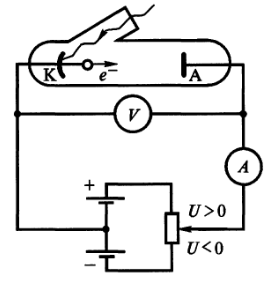
\includegraphics[width=0.8\textwidth]{img/oral-05/photoel.png}
  \label{fig:photoel}
\end{figure}

\begin{figure}[h]
  \centering
  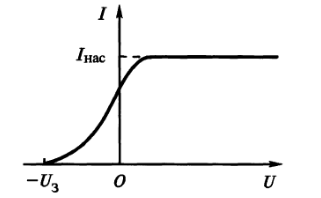
\includegraphics[width=0.8\textwidth]{img/oral-05/vah.png}
  \caption{ВАХ}
  \label{fig:vah}
\end{figure}

При положительном напряжении электрическое поле ускоряет электрон и все
электроны достигают анода, создавая \emph{фототок насыщения} $ I_k $.

Небольшой спад фототока при малых положительных 
напряжениях, который наблюдается в опытах, связан с контактной 
разностью потенциалов между катодом и анодом. Далее при 
обсуждении закономерностей фотоэффекта мы будем пренебрегать
влиянием контактной разности потенциалов.

При $ U < 0 $ не все электроны могут достичь анод, а лишь те, у которых
достаточно кинетической энергии. По графику видно, что она встречается разная.
\emph{Задерживающим напряжением} $ U_{\text{З}} $ назовём такое, при котором
фототок равен нулю.

Измерим $ U_{\text{З}} $ и определим максимальную энергию электрона из
соотношения\footnote{При рассмотрении, например, рентгеновского или $ \gamma $
излучения следует перейти к релятивистской формуле.} 
\[
  E_m = \frac{1}{2}m_0 v_m^2 = eU_{\text{З}}.
\]

Экспериментально были установлены следующие \emph{законы фотоэффекта}:
\begin{enumerate}
  \item Для монохроматического света определенной длины волны
фототок насыщения пропорционален световому потоку, 
падающему на катод.
\item Максимальная кинетическая энергия фотоэлектронов не 
зависит от величины светового потока, а определяется лишь 
частотой излучения.
\item Для каждого вещества катода существует своя граничная
частота $ \nu_K $, такая, что излучение с частотой $ \nu < \nu_K $ фотоэффекта
не вызывает. Эту граничную частоту называют частотой красной
границы фотоэффекта. По шкале длин волн ей соответствует 
длина волны красной границы $ \lambda_K $, такая, что эмиссию электронов из
данного металла вызывает излучение лишь с меньшей длиной
волны ($ \lambda < \lambda_K $).
\end{enumerate}

Классическое рассмотрение проваливается, поскольку, например, должен нарушаться
второй закон, поскольку электроны в этой теории вылетают засчёт силы
электромагнитного поля.

Эйнштейн предложил концепцию фотонов как частиц
излучения, несущих квант энергии. Действительно, в таком
процессе электрон получает всю энергию от фотона, которая 
пропорциональна частоте излучения. Число же вырванных из металла
электронов и, следовательно, фототок насыщения пропорциональны числу падающих на
металл фотонов, которое определяется
величиной потока энергии излучения. Тогда из закона сохранения энергии для
электронов, которым нужно проделать пренебрежимо малую работу для достижения
границы, справедлива формула  
\[
    h\nu = A_B + E_m.
\]
Непосредственно из этого уравнения вытекают второй и третий законы фотоэффекта.
Получаем простые формулы для частоты/длины волны красной границы. Они полностью
определяются $ A_B $.

Возражение о том, что свободный электрон не может поглотить фотон легко
парируется тем фактом, что <<свободные>> электроны в металле взаимодействуют с
атомами решётки.

Назовём \emph{квантовым выходом} $ Y $ число вылетивших электронов на один
падающий фотон. Вблизи красной границы для большинства металлов $ Y = 10^{-4} $
электрон/фотон. Малость квантого выхода обусловлена требованием близости
электронов к границе --- не более $ 0.1 $ мкм. Кроме того, поверхность металлов
сильно отражает излучение. С увеличением энергии фотонов (частоты) $ Y \approx
0.01 \ldots 0.05 $ электрон/фотон. 

С помощью фотоэффекта можно оценить значение $ h $. Для этого запишем уравнение Эйнштейна
в виде 
\[
  eU_{\text{З}} = h\nu - A_B
\]
и увидим, что $ U_{\text{З}} $ линейно зависит от $ \nu $ с угловым
коэффициентом $ h $.

Приборы, в основе устройства которых лежит фотоэффект, 
называют фотоэлементами. Обычный вакуумный фотоэлемент 
выполнен в виде вакуумированной колбы, у которой внутреннюю
поверхность, за исключением небольшого окошечка для доступа
света, покрывает тонкая пленка из металла с малой работой 
выхода (цезий, калий, натрий). Анод представляет собой проволочное
кольцо в центре колбы. Между катодом и анодом прикладывается
ускоряющее напряжение 80\ldots100 В. Фотоэлементы широко 
применяются в технике (фотореле, люксметры, системы звукозаписи
на пленку и др.).


\subsubsection{Комптон-эффект}
При большой энергии излучения поглощение фотонов электронами становится
маловероятным. Здесь при взаимодействии излучения с веществом наблюдается
рассеяние излучения.

Схематически экспериментальная установка Комптона 
изображена на рис. \ref{fig:kompton}. Рентгеновская трубка РТ была смонтирована
на вращающейся платформе, что позволяло при ее повороте 
изменять угол рассеяния $ \theta $ рентгеновского излучения, попадающего
после мишени-рассеивателя в измерительный блок установки.

\begin{figure}[h]
  \centering
  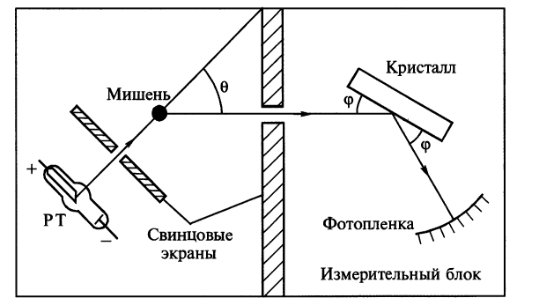
\includegraphics[width=0.8\textwidth]{img/oral-05/kompton}
  \label{fig:kompton}
\end{figure}

Длина волны рассеянного излучения определялась с помощью
дифракции его на кристалле. Согласно дифракционной теории,
при выполнении условия Брэгга -- Вульфа 
\[
    2d\sin\varphi = n\lambda', \quad n = 1,2, \ldots,
\]
где $ d $ --- расстояние между атомными плоскостями кристалла, а $ \varphi $ ---
угол скольжения падающего излучения, наблюдается 
интенсивное отражение от кристалла рассеянного рентгеновского излучения.
Поэтому, зная параметры кристаллической решетки $ d $, и измерив
угол $ \varphi $ для максимума отражения $ n $-го порядка, можно рассчитать
длину волны $ \lambda' $ рентгеновского излучения, рассеянного мишенью.
Соответствие угла $ \varphi $ и длины волны $ \lambda' $, вытекающее из формулы
выше, 
позволяло нанести на фотопленку шкалу длин волн и по положению
на фотопленке засвеченной полоски определить длину волны 
рассеянного рентгеновского излучения. В первых опытах Комптона 
вместо фотопленки использовалась подвижная ионизационная камера,
позволяющая по значению тока в приборе фиксировать отраженное
от кристалла рентгеновское излучение.

Экспериментально определено, что разность длин волн зависит только от угла $
\theta $: 
\[
    \Delta \lambda = \lambda' - \lambda = \Lambda_K (1-\cos\theta),
\]
где $ \Lambda_K = 2.426\times10^{-12} $ м.

С точки зрения классической физики этот эффект необъясним. Там рассеяние можно
рассматривать как вынужденые колебания электронов (под действием силы
электромагнитных волн), и излучение им вторичных рассеяных волн, но на той же
частоте.

В квантовой оптике этот эффект объясняется как следствие упругого рассеяния
фотона $ \Phi \to \Phi' $ на свободном электроне вещества (см. рис.
\ref{fig:compton2}). Формула Комптона тогда есть следствие законов сохранения
энергии и импульса.

\begin{figure}[H]
	\begin{center}
		\begin{tikzpicture}[thick]
			\begin{scope}
				\path [draw=blue,snake arrow,->]
				(-4,0) -- (-2,0) node[anchor=south]{\hspace{-2cm}$h\nu$};
				\filldraw[black] (-1,0) circle (2pt) node[anchor=north]{$\vec e$};
			\end{scope}
			$\implies$
			\begin{scope}
				\path [draw=blue,dashed] (1,0)--(4,0);
				\path [draw=blue,snake arrow,->]
				(2,0) -- (3.5,1) node[anchor=east]{\hspace{-2cm}$h\nu'$};
				\path [draw=black, ->]
				(2,0) -- (2.5,-1) node[anchor=west]{$\vec p_e$};
				\draw[black] (3,0) arc (0:31:1) node[anchor=west]{$\theta$};
			\end{scope}
		\end{tikzpicture}
	\end{center}
	\caption{Комптон-эффект}
  \label{fig:compton2}
\end{figure}

Действительно, $ E = h\nu = (hc)/\lambda $ и закон сохранения энергии принимает
вид
\[
    \frac{hc}{\lambda} + m_0c^2 = \frac{hc}{\lambda'} + mc^2.
\]
Здесь $ m = \gamma m_0 $, $ \gamma = (1-v^2/c^2)^{-1/2} $ --- релятивистский
множитель. Уже сейчас видно, что $ \lambda' > \lambda $.

Закон сохранения импульса принимает вид 
\[
    \hbar \mathbf k = \hbar \mathbf k' + m \mathbf v,
\]
откуда, учитывая $ k = 2\pi/\lambda $,
\[
  (mv)^2 = \left( \frac{h}{\lambda} \right)^2  + \left( \frac{h}{\lambda'}
  \right)^2 - 2 \frac{h^2}{\lambda \lambda'}\cos\theta.
\]

\begin{figure}[H]
	\begin{center}
		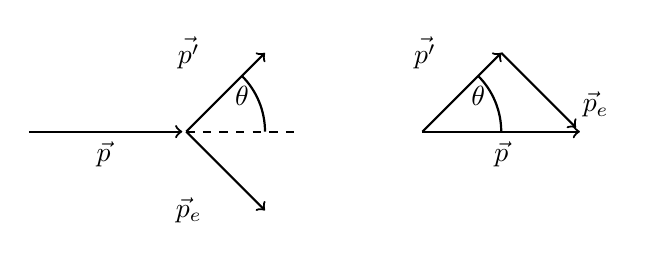
\begin{tikzpicture}[thick]
			\begin{scope}
				\path[draw=black,->] (-2,0)--(-0.05,0) node[anchor=north]{\hspace{-2cm}$\vec p$};
				\path[draw=black,->] (0,0)--(1,1) node[anchor=west]{\hspace{-2cm}$\vec {p'}$};
				\path[draw=black,->] (0,0)--(1,-1) node[anchor=west]{\hspace{-2cm}$\vec p_e$};
				\draw[black] (1,0) arc (0:45:1) node[anchor=north]{$\theta$};
				\path[draw=black,dashed] (0,0)--(1.4,0) ;
			\end{scope}
			%			$\Leftrightarrow$
			\begin{scope}
				\path[draw=black,->] (3,0)--(5,0) node[anchor=north]{\hspace{-2cm}$\vec p$};
				\path[draw=black,->] (3,0)--(4,1) node[anchor=west]{\hspace{-2cm}$\vec {p'}$};
				\path[draw=black,->] (4,1)--(4.95,0.05) node[anchor=south]{\hspace{0.5cm}$\vec p_e$};
				\draw[black] (4,0) arc (0:45:1) node[anchor=north]{$\theta$};
			\end{scope}
		\end{tikzpicture}
	\end{center}
	\caption{Закон сохранения импульса}
\end{figure}

Преобразуем теперь закон сохранения энергии к виду  
\begin{align*}
  mc &= m_0 c + \frac{h}{\lambda} - \frac{h}{\lambda'},\\
  (mc)^2 &= (m_0c)^2 + 2m_0ch \left( \frac{1}{\lambda} - \frac{1}{\lambda'}
  \right) + \left( \frac{h}{\lambda} \right)^2 - \frac{2h^2}{\lambda\lambda'} +
  \left( \frac{h}{\lambda'} \right)^2.
\end{align*}
Из соотношения $ (mc)^2 - (m_0c)^2 = (mv)^2 $ выразим соответствующим образом $
mv $ и объединим законы сохранения формулой 
\[
    2m_0 ch \left( \frac{1}{\lambda} - \frac{1}{\lambda'} \right) =
    \frac{2h^2}{\lambda\lambda'}(1-\cos\theta).
\]
Отсюда и получаем формулу Комптона  
\[
    \lambda' - \lambda = \frac{}{}
\]



\subsubsection{Дифракция электронов (в чем отличие от дифракции рентгеновских лучей?)}
\begin{itemize}
	\item Опыт Девисона-Джермера (монокристалл);
	\item Опыты Томсона и Тартаковского (поликристалл);
	\item Опыт Фабриканта (одиночные электроны);
\end{itemize}
\newpage
\paragraph{Опыт Девисона-Джермера (монокристалл)}
\begin{wrapfigure}{r}{0.5\linewidth}
	\centering
	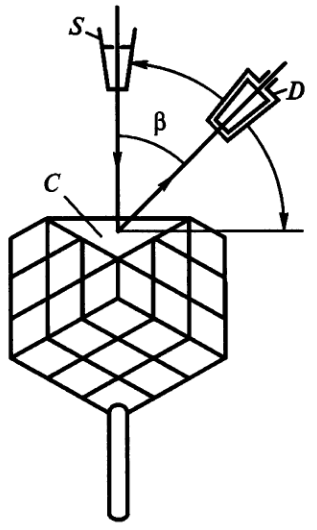
\includegraphics[width=0.5\linewidth]{img/oral-05/devison-djermer}
	\caption{Схема опыта Девисона-Джермера}
	\label{fig:devison-djermer}
\end{wrapfigure}
Электроны от электронной пушки $S$, прошедшие ускоряющую разность потенциалов $U$, падали нормально на сошлифованную поверхность кристалла никеля $C$. С помощью детектора $D$ исследовалось число электронов, отраженных от кристалла под углом $\beta$ при различных значениях $U$. Напомним, что разным значениям $U$ соответствуют разные дебройлевские длины волн электронов.

В опытах наблюдалось максимальное отражение электронов при ускоряющей разности потенциалов $U=54$ В (см. Рис \ref{fig:devison-djermer-electron-difraction-dynamics}), что соответсвует дебройлевской длине волны
\begin{equation*}
	\lambda_{\text{Б}}=\frac{2\pi\hbar}{\sqrt{2m_eeU}}=0.167 \text{нм}
\end{equation*}

Из условия Брэгга-Вульфа 
\begin{equation*}
	2d\sin\theta=n\lambda_{\text{Б}}
\end{equation*}
для постоянной решетки никеля $d=2.15\cdot10^{-10}$ определяется, <<теоретическая>> дебройлевская длина волны, она равняется $\lambda_{\text{Б}}=0.165$ нм, что отлично соотносится с результатами опыта и служит подтверждением гипотезы де Бройля.

\begin{figure}[H]
	\centering
	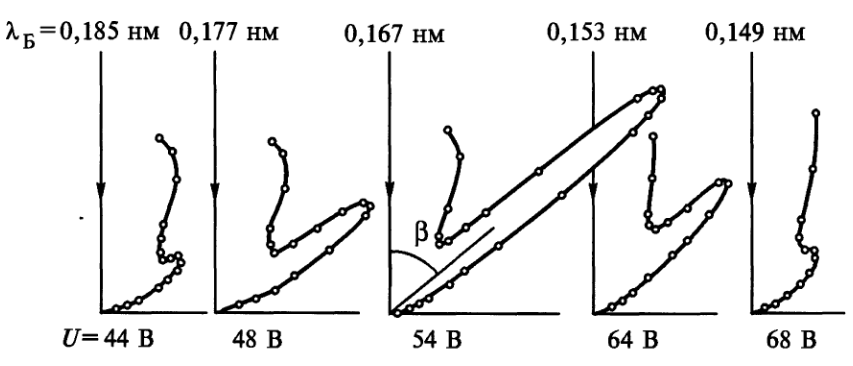
\includegraphics[width=0.8\linewidth]{img/oral-05/devison-djermer-electron-difraction-dynamics}
	\caption{Динамика дифракционного отражения электронов при изменении ускоряющей разности потенциалов $U$}
	\label{fig:devison-djermer-electron-difraction-dynamics}
\end{figure}

Была также измерена интенсивность дифрагирующих электронов в зависимости от ускоряющей разности потенциалов $U$ (см. Рис \ref{fig:devison-djermer-intensivnost-u}). Максимумы остоят друг от друга на равном по шкале $\sqrt{U}$ расстоянии, что подтверждается теорией.
\begin{equation*}
	\lambda_{\text{Б}}=\frac{2\pi\hbar}{\sqrt{2m_eE_k}}=\frac{2\pi\hbar}{\sqrt{2m_eeU}}\implies2d\sin\theta=n\frac{2\pi\hbar}{\sqrt{2m_eeU_n}},
\end{equation*}
где $U_n$ --- ускоряющая разность потенциалов, соответствующая $n$-му порядку отражения.

Таким образом связь между $U_n$ и $n$ имеет вид
\begin{equation*}
	\sqrt{U_n}=Cn,\,\text{где}\: C=\frac{\pi\hbar}{d\sin\theta\sqrt{2em_e}}=\mathrm{const}
\end{equation*}

\begin{figure}[H]
	\centering
	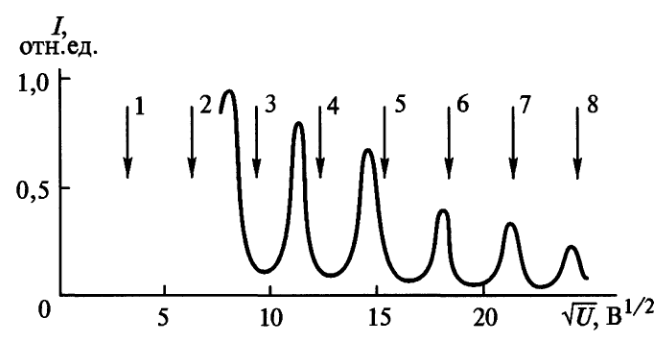
\includegraphics[width=0.6\linewidth]{img/oral-05/devison-djermer-intensivnost-u}
	\caption{Зависимость интенсивности $I$ пучка электронов, дифрагирующего на монокристалле никеля, от ускоряющего напряжения $U$ при постоянном значении угла $\theta$}
	\label{fig:devison-djermer-intensivnost-u}
\end{figure}
Различие теории и эксперимента в этом опыте заключалось в том, что положения наблюдаемых дифракционных максимумов не совпадали с положениями максимумов, определяемых из условия Брэгга — Вульфа (вертикальные стрелки на Рис. \ref{fig:devison-djermer-intensivnost-u}). Особенно заметным это различие было для небольших значений $n$, т. е. для небольшой ускоряющей разности потенциалов $U_n$. Причина такого расхождения теории и эксперимента состоит в том, что условие Брэгга — Вульфа не учитывает преломление электронных волн в металле. 
Использование условия с поправкой на преломление внутри кристалла:
\begin{equation*}
	2d\sqrt{n_e^2-\cos^2\theta}=n\lambda_{\text{Б}}
\end{equation*}
полностью устраняет это расхождение.

\paragraph{Опыты Томсона и Тартаковского (поликристалл)}
В результате наблюдале концентрические кольца, которые хорошо описывались условиями Брэгга-Вульфа
\begin{equation*}
	2d\sin\theta=n\lambda_{\text{Б}},\: R=L\tg2\theta
\end{equation*}
\begin{multicols}{2}
	\begin{figure}[H]
		\centering
		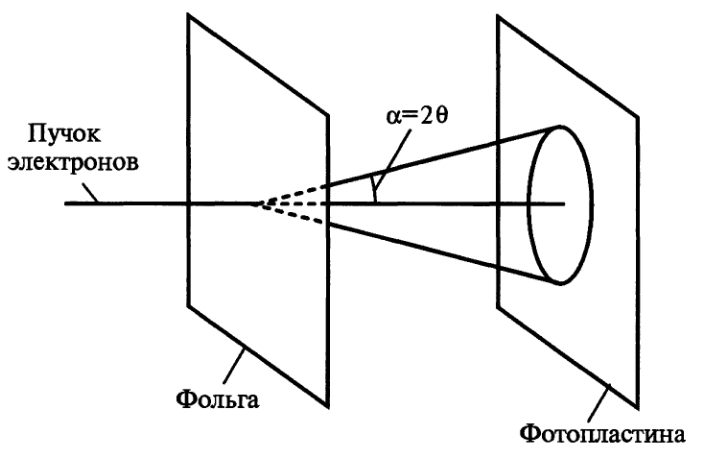
\includegraphics[width=\linewidth]{img/oral-05/tomson-tartakovsky}
		\caption{Дифракция электронов в поликристаллической фольге}
		\label{fig:tomson-tartakovsky}
	\end{figure}
	\begin{figure}[H]
		\centering
		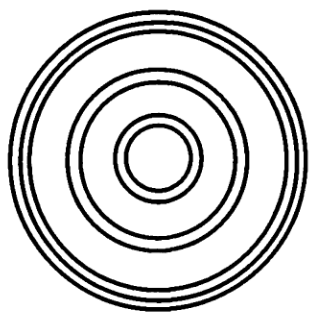
\includegraphics[width=0.64\linewidth]{img/oral-05/tomson-tartakovsky-results}
		\caption{Результаты дифракционных опытов с электронами на поликристалле серебра}
		\label{fig:tomson-tartakovsky-results}
	\end{figure}
\end{multicols}

Добавление магнитного поля между фольгой и экраном позволило подтвердить, что происходит дифракция именно электронов.

\newpage
\paragraph{Опыт Фабриканта (одиночные электроны)}
В этих опытах промежуток времени между двумя последовательными прохождениями электронов через кристалл в 30 000 раз превышал время, затрачиваемое одним электроном на прохождение всего прибора. Таким образом, электроны дифрагировали в кристалле поодиночке, поэтому возникновение дифракционной картины как результата взаимодействия электронов друг с другом полностью исключалось.

Качественный вид распределения дифрагировавших электронов по фотопластинке приведен на Рис. \ref{fig:fabrikant-results}. При небольшой длительности эксперимента точки на фотопластинке, отвечающие попаданию электронов, распределены совершенно случайным образом (Рис. \ref{fig:fabrikant-results}, а). 

Однако при достаточной длительности эксперимента распределение точек приобретает характерный для дифракции на поликристалле вид концентрических колец (Рис. \ref{fig:fabrikant-results}, б). Таким образом было доказано, что волновые свойства присущи отдельному электрону.
\begin{figure}[H]
	\centering
	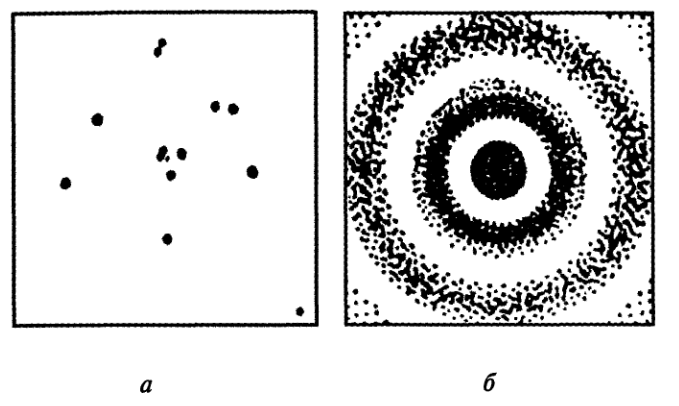
\includegraphics[width=0.7\linewidth]{img/oral-05/fabrikant-results}
	\caption{Распределение дифрагирующих электронов по фотопластинке \\ a --- при небольшой длительности эксперимента;\\б --- в случае длительного эксперимента;}
	\label{fig:fabrikant-results}
\end{figure}



\subsubsection{Опыт Штерна-Герлаха}
Ниже (см. магнетон Бура) доказано соотношение 
\[
  p^M_z = \Gamma_0L_z = m\mu_{\text{Б}},
\]
где $ m $ --- магнитное квантовое число, $ p^M $ --- магнитный момент. Эта
формула говорит о дискретности проекции магнитного момента атома на выделенное
направление $ z $ внешнего магнитного поля.

Попробуем доказать или опровергнуть это утверждение эмпирически. Поставим
вакуумную печь, куда положим атомы, например, серебра. Труба у этой печи будет
столь тонкой, что сформируется узкий атомный пучок. Этот пучок пропускают через
неоднородное 
магнитное поле с существенным градиентом магнитной индукции. 
Индукция магнитного поля $ \mathbf B $ в опыте достаточно велика и направлена
вдоль оси $ z $.

Для создания такого магнитного поля используют магнит с но-
жевидным полюсным наконечником вблизи которого проходит
атомный пучок (рис. \ref{fig:puchok}, б).

\begin{figure}[h]
  \centering
  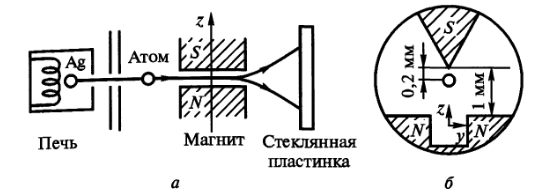
\includegraphics[width=0.8\textwidth]{img/oral-05/puchok.png}
  \label{fig:puchok}
\end{figure}

На пролетающие в зазоре магнита атомы вдоль направления магнитного поля
действует сила  
\[
    F_z = p_z^M \frac{\partial B}{\partial z},
\]
обусловленная градиентом индукции неоднородного магнитного
поля и зависящая от значения проекции магнитного момента 
атома на направление поля. Эта сила отклоняет движущийся атом в
направлении оси $ z $, причем за время пролета магнита движущийся
атом отклоняется тем больше, чем больше сила $ F_z $. При этом одни
атомы отклоняются вверх, а другие --- вниз. Посмотрим на полученную картину на
стеклянной пластинке. Вместо непрерывной зеркальной линии, которая должна была бы
получиться согласно классической физике (ведь тепловое движение хаотично), имеем серию узкиъ зеркальных полосок из
напыленных атомов.


